\section{Noise removal}


\begin{figure}[!htbp]
\minipage{.47\textwidth}%
\centering
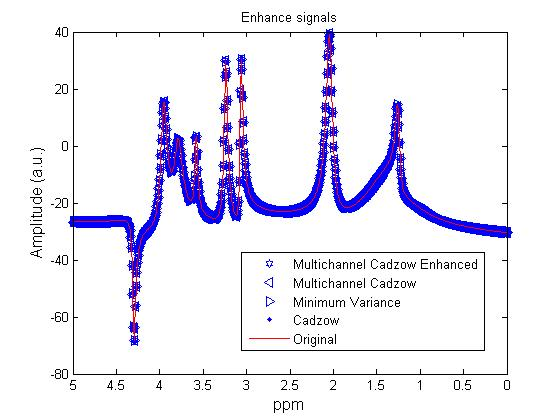
\includegraphics[width=1\textwidth]{27.jpg}
\subcaption{Original signal and its respective enhancement after Cadzow, Minimum variance, Multichannel Cadzow, and Enhanced Multichannel Cadzow}
\endminipage\hfill
\minipage{.47\textwidth}%
\centering
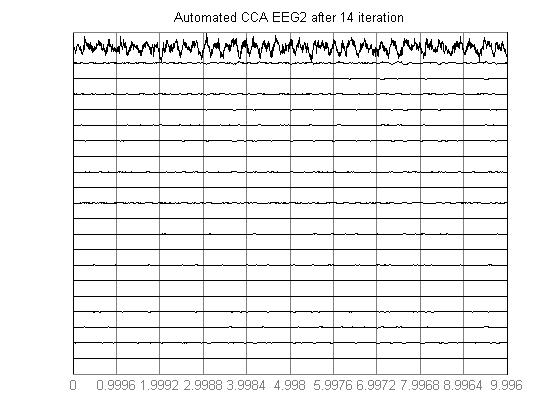
\includegraphics[width=1\textwidth]{28.jpg}
\subcaption{Original signal and its respective estimation after Cadzow, Minimum variance, Multichannel Cadzow, and Enhanced Multichannel Cadzow enhancement}
\endminipage\hfill
\caption{Enhancement of the signal employing both single channel and multichannel approach}
\end{figure}

Hereby different enhancement techniques are being investigated. Starting with the Cadzow technique which consist of a simple truncation of the singular values decomposition method. Meaning that the low singular values (low level of information) is canceled out due to its inferior contribution to the spectrum of interest.

Minimum variance in addition in addition to truncation tries to decrease the residue of the singular values with an arbitrary value as:

\begin{equation}
\sigma_{i}=\sigma_{i}-\sigma_{r}
\end{equation}

where $\sigma_{r}$ in our implementation consist of the average of the dropped singular values dropped by the truncation\cite{11}. This could also be the smalles value of the singuar matrix which has been used in other implementation\cite{2}. This method indicates a very small SNR improvement. This far it was only taken into the consideration the single channel enhancement technique. When neighbouring of the main voxels with the distance of 3x3 voxel are taken into account an significant improvement of the signal to noise ration has been investigated. In the figure \ref{figtoda1} there is an overview of the voxel of interest together with its 9x9 neighbours. In the first implementation, 9 signals are taken into a neighbourhood of 3x3 voxels where the main voxel is the region of the interest. Then each of the signal is reshaped into an Hankel matrix thus 9 matrices in total. These matrices are then merged horizontally one by one to creating a array of matrices and the final matrix consist of the signal to be proceeded. SVD is computed from this matrix which is a very heavy computation. A model order of 30 has been incorporated into this computation, meaning that truncation after the SVD will take only the first 30 singular values. After the truncation the matrix of our interest which contain the signal of the main voxel is picked up and average along the anti-diagonal. The result is another Hankel matrix where after reshaping the matrix into the original signal dimension and much higher SNR has been observed. Some important remarks are: ordering of the signals when the Hankel matrices are merged does not influence the result \cite{14}. The model order is fixed and there is only one step of performed for this estimation. 

However the multichannel method is further improved by taking different order of the model and by taking different distance of the neighbours. Starting with a 3x3 neighbours and moving into 5x5,7x7, and 9x9. This is first performed along the horizontal and vertical neighbours then along the diagonal and anti-diagonal neighbours. Whereas due to the memory complexity and limited resources it was not possible to run with full neighbourhoods at scale higher than 5x5. It has been observed that SNR tends to decay for higher neighbourhood for lower model order. Thus it was decided to not run the full neighbourhood model since from the 5x5 SNR is lower than 3x3. Moreover this goes the same for the other two neigbhourhooding.  


Starting with the water filter signal where its SNR is \textbf{\textit{$-25.2546 dB$}} Cadzow outcomes an significant improvement of the SNR up to $3.7264 dB$. Minimum variance implementation tends to be slightly higher compare to Cadzow nevertheless is still an improvement with is translated into lower level of noise. Further more the noise suppression is far higher in the multichannel case where $3x3$ voxel will yield an SNR of $39.5513$ whereas $5x5$ voxel case will yield a slightly lower SNR of $38.5198 dB$. Since the SNR decays as the number of neighbours voxels increases SNR tends to decays thus there was no encouragement in testing the ordinary Multichannel Cadzow despite its memory and time complexity which is technically NP. Since time complexity is a more desirable  compare to memory complexity.  Even though both are bad scenario memory requires physical resources whereas time could be achieved by just waiting. 
The best performance is achieved with vertically and horizontally neighbours at order of 22 with 3x3 voxels with a SNR of \textbf{\textit{$40.1137 dB$}}. This method however performs better compare to the diagonal and anti-diagonal version   respectively to model order and voxels range. This could be concluded from the table \ref{niceday} and table \ref{niceday1}. Further more for the cases of 3x3 and 5x5 range the generic Multichannel Cadzow tends to be higher compare to the anti-diagonal case however is still inferior to the horizontal and vertical case.


%%%%%%%%%%%%%%%%%%%%%%%%%%%%%%%%%%%%%%%%%%%%%%%%%%%%%%%%%%%%%%%%%%%%%%%%%%%%%%%%%%%%%%%%%%%%%%%%%%%%%%%%%%%%%%%%%%%%%%%%%%%%%%%%%%%%%%%%%%%%%%%%%%%%%%%%%%%%%%%%%%%%%%%%%%%%%%%%%%%%%%%%%%%%


\begin{table}[!htbp]
\centering
\caption{Signal to noise values for the anti diagonal and diagonal neighbours at $dB$ level. Different model are tested further more using different neighbouring range}\label{niceday}
\label{table:55}
\begin{tabular}{c c c c c c c c c c c c c c c c c}
  \hline  
$K$&$30$&$29$&$28$&$27$&$26$&$25$&$24$&$23$&$22$&$21$&$20$\\
  \hline  
$3x3$&$36.2700$&$37.7028$&$36.0013$&$35.8031$&$35.4027$&$35.7358$&$35.7531$&$35.4922$&$37.1925$&$37.6473$&$37.6407$\\
$5x5$&$36.4102$&$37.7397$&$36.0068$&$35.9564$&$35.3598$&$35.7904$&$35.6169$&$35.7460$&$37.1497$&$37.6843$&$37.7884$\\
$7x7$&$36.1939$&$37.7153$&$35.9040$&$36.0002$&$35.3396$&$35.8426$&$35.5035$&$35.7533$&$37.1429$&$37.6568$&$37.7309$\\
$9x9$&$35.8524$&$36.9298$&$35.7412$&$36.1220$&$35.3127$&$35.9223$&$35.5232$&$35.7155$&$37.1599$&$37.8243$&$37.5072$\\
  \hline  
\end{tabular}
\end{table}  
  
  
  \begin{table}[!htbp]
\centering
\caption{Signal to noise values for the  vertical and horizontal neighbours at $dB$ level. Different model are tested further more using different neighbouring range}\label{niceday1}
\label{table:55}
\begin{tabular}{c c c c c c c c c c c c c c c c c} 
  \hline  
$K$&$30$&$29$&$28$&$27$&$26$&$25$&$24$&$23$&$22$&$21$&$20$\\
  \hline  
$3x3$&$40.0829$&$39.1976$&$37.6684$&$37.0776$&$36.1116$&$37.5342$&$35.8595$&$34.8111$&\textbf{\textit{$40.1137$}}&$38.0277$&$37.6797$\\
$5x5$&$38.1118$&$36.5473$&$37.0211$&$36.7936$&$35.2903$&$35.2727$&$34.9380$&$34.8007$&$37.4030$&$36.6630$&$33.8714$\\
$7x7$&$36.7022$&$36.5759$&$37.0355$&$36.5761$&$35.0747$&$35.1001$&$34.9214$&$34.7472$&$37.4039$&$36.6613$&$33.8988$\\
$9x9$&$36.9532$&$36.6120$&$37.0117$&$36.4066$&$35.0171$&$35.1019$&$34.8839$&$34.7718$&$37.3859$&$36.5159$&$33.9277$\\
 \hline
\end{tabular}
\end{table}



 \begin{table}[!htbp]
\centering
\caption{Frequency estimation \textbf{\textit{Hz}}}
\label{table:5}
\begin{tabular}{c c c c c c c c c c c c c c c c c c c c c c c c c c c c c c c } 
   \hline 
$Signals$&$Pure$&$Cdz$&$MinVar$&$MultiCh$&$OptiMultiCha$\\
   \hline 

$1$&$ 0.9079$&$ 0.9127$&$ 0.8988$&$-0.0129$&$-0.0127$\\
$2$&$ 0.8004$&$ 0.7810$&$ 0.6782$&$-0.0151$&$-0.0129$\\
$3$&$ 0.6815$&$ 0.7116$&$ 0.2674$&$-0.0160$&$-0.0162$\\
$4$&$ 0.2310$&$ 0.2280$&$-0.0128$&$-0.0257$&$-0.0507$\\
$5$&$-0.0128$&$-0.0128$&$-0.0508$&$-0.0506$&$-0.0630$\\
$6$&$-0.0508$&$-0.0508$&$-0.0949$&$-0.0700$&$-0.0951$\\
$7$&$-0.0949$&$-0.0949$&$-0.0954$&$-0.0954$&$-0.1143$\\
$8$&$-0.0954$&$-0.0954$&$-0.1168$&$-0.1119$&$-0.1148$\\
$9$&$-0.1168$&$-0.1168$&$-0.1429$&$-0.1424$&$-0.1427$\\
$10$&$-0.1429$&$-0.1429$&$-0.1645$&$-0.1623$&$-0.1632$\\
$11$&$-0.1645$&$-0.1645$&$-0.1863$&$-0.1679$&$-0.1634$\\
$12$&$-0.1863$&$-0.1863$&$-0.1903$&$-0.1704$&$-0.1636$\\
$13$&$-0.2085$&$-0.2082$&$-0.2085$&$-0.1731$&$-0.1651$\\
$14$&$-0.2166$&$-0.2085$&$-0.3137$&$-0.1864$&$-0.1863$\\
$15$&$-0.3144$&$-0.3169$&$-0.3396$&$-0.2085$&$-0.2085$\\
$16$&$-0.3239$&$-0.3396$&$-0.3441$&$-0.2920$&$-0.2653$\\
$17$&$-0.3396$&$-0.3578$&$-0.4273$&$-0.3385$&$-0.3396$\\
$18$&$-0.3825$&$-0.4273$&$-0.4409$&$-0.4226$&$-0.3956$\\
$19$&$-0.4273$&$-0.4409$&$-0.4576$&$-0.4234$&$-0.4229$\\
$20$&$-0.4409$&$-0.4972$&$-0.4647$&$-0.4387$&$-0.4406$\\
$21$&$-0.6682$&$-0.9445$&$-0.9371$&$-0.4818$&$-0.4776$\\
$22$&$-0.9445$&$-0.9996$&$-0.9445$&$-0.9535$&$-0.9429$\\
     \hline 

\end{tabular}
\end{table}

 \begin{table}[!htbp]
\centering
\caption{Damping estimation \textbf{\textit{Hz}}}
\label{table:5}
\begin{tabular}{c c c c c c c c c c c c c c c c c c c c c c c c c c c c c c c } 
   \hline 
$Signals$&$Pure$&$Cdz$&$MinVar$&$MultiCh$&$OptiMultiCha$\\
   \hline 
$1$&$ 4.0342$&$ 4.0342$&$ 4.1211$&$ 3.9398$&$ 3.9937$\\
$2$&$ 0.5761$&$ 1.2324$&$ 4.0342$&$ 0.1416$&$ 0.3137$\\
$3$&$ 0.5179$&$ 0.8633$&$ 0.7609$&$ 0.0689$&$ 0.2699$\\
$4$&$ 0.3748$&$ 0.7635$&$ 0.4569$&$ 0.0610$&$ 0.1916$\\
$5$&$ 0.2642$&$ 0.3748$&$ 0.3748$&$ 0.0548$&$ 0.1731$\\
$6$&$ 0.2633$&$ 0.2633$&$ 0.2633$&$ 0.0539$&$ 0.1129$\\
$7$&$ 0.1784$&$ 0.2361$&$ 0.1900$&$ 0.0322$&$ 0.0823$\\
$8$&$ 0.0829$&$ 0.1674$&$ 0.1446$&$ 0.0259$&$ 0.0762$\\
$9$&$ 0.0700$&$ 0.0700$&$ 0.1082$&$ 0.0253$&$ 0.0613$\\
$10$&$ 0.0407$&$ 0.0617$&$ 0.1012$&$ 0.0226$&$ 0.0357$\\
$11$&$ 0.0378$&$ 0.0497$&$ 0.0740$&$ 0.0172$&$ 0.0318$\\
$12$&$ 0.0355$&$ 0.0396$&$ 0.0700$&$ 0.0146$&$ 0.0262$\\
$13$&$ 0.0351$&$ 0.0355$&$ 0.0477$&$ 0.0135$&$ 0.0202$\\
$14$&$ 0.0303$&$ 0.0303$&$ 0.0355$&$ 0.0085$&$ 0.0160$\\
$15$&$ 0.0246$&$ 0.0246$&$ 0.0303$&$ 0.0077$&$ 0.0155$\\
$16$&$ 0.0205$&$ 0.0202$&$ 0.0246$&$ 0.0069$&$ 0.0152$\\
$17$&$ 0.0202$&$ 0.0174$&$ 0.0202$&$ 0.0053$&$ 0.0146$\\
$18$&$ 0.0174$&$ 0.0153$&$ 0.0174$&$ 0.0052$&$ 0.0144$\\
$19$&$ 0.0153$&$ 0.0149$&$ 0.0153$&$ 0.0041$&$ 0.0095$\\
$20$&$ 0.0149$&$ 0.0106$&$ 0.0149$&$ 0.0040$&$ 0.0048$\\
$21$&$ 0.0094$&$ 0.0094$&$ 0.0094$&$ 0.0028$&$ 0.0020$\\
$22$&$ 0.0012$&$ 0.0012$&$ 0.0012$&$ 0.0020$&$-0.0041$\\
     \hline 

\end{tabular}
\end{table}

 \begin{table}[!htbp]
\centering
\caption{Amplitude estimation \textbf{\textit{a.u}}}
\label{table:5}
\begin{tabular}{c c c c c c c c c c c c c c c c c c c c c c c c c c c c c c c } 
   \hline 
$Signals$&$Pure$&$Cdz$&$MinVar$&$MultiCh$&$OptiMultiCha$\\
   \hline 
$1$&$32.9413$&$32.9413$&$32.9413$&$32.8043$&$32.8789$\\
$2$&$ 2.3434$&$ 2.3434$&$ 2.3434$&$ 1.2190$&$ 1.1372$\\
$3$&$ 1.3716$&$ 1.3716$&$ 1.3716$&$ 1.1237$&$ 1.1268$\\
$4$&$ 1.1270$&$ 1.1270$&$ 1.1270$&$ 0.8893$&$ 1.0544$\\
$5$&$ 0.8892$&$ 0.8892$&$ 0.8892$&$ 0.8106$&$ 1.0370$\\
$6$&$ 0.5870$&$ 0.5870$&$ 0.5870$&$ 0.7964$&$ 0.8976$\\
$7$&$ 0.5632$&$ 0.5632$&$ 0.5632$&$ 0.6668$&$ 0.6491$\\
$8$&$ 0.4281$&$ 0.4281$&$ 0.4281$&$ 0.5959$&$ 0.5619$\\
$9$&$ 0.3526$&$ 0.3526$&$ 0.3526$&$ 0.5087$&$ 0.4340$\\
$10$&$ 0.3135$&$ 0.3135$&$ 0.3135$&$ 0.3115$&$ 0.3726$\\
$11$&$ 0.2800$&$ 0.2800$&$ 0.2800$&$ 0.1996$&$ 0.2987$\\
$12$&$ 0.2206$&$ 0.2206$&$ 0.2206$&$ 0.1851$&$ 0.2743$\\
$13$&$ 0.0051$&$ 0.0051$&$ 0.0051$&$ 0.0841$&$ 0.1752$\\
$14$&$ 0.0000$&$ 0.0000$&$ 0.0000$&$ 0.0658$&$ 0.0888$\\
$15$&$ 0.0000$&$ 0.0000$&$ 0.0000$&$ 0.0381$&$ 0.0677$\\
$16$&$ 0.0000$&$ 0.0000$&$ 0.0000$&$ 0.0288$&$ 0.0616$\\
$17$&$ 0.0000$&$ 0.0000$&$ 0.0000$&$ 0.0204$&$ 0.0610$\\
$18$&$ 0.0000$&$ 0.0000$&$ 0.0000$&$ 0.0140$&$ 0.0190$\\
$19$&$ 0.0000$&$ 0.0000$&$ 0.0000$&$ 0.0075$&$ 0.0190$\\
$20$&$ 0.0000$&$ 0.0000$&$ 0.0000$&$ 0.0070$&$ 0.0091$\\
$21$&$ 0.0000$&$ 0.0000$&$ 0.0000$&$ 0.0040$&$ 0.0002$\\
$22$&$ 0.0000$&$ 0.0000$&$ 0.0000$&$ 0.0037$&$ 0.0000$\\
     \hline 

\end{tabular}
\end{table}

 \begin{table}[!htbp]
\centering
\caption{Phase estimation \textbf{\textit{Deg}}}
\label{table:5}
\begin{tabular}{c c c c c c c c c c c c c c c c c c c c c c c c c c c c c c c } 
   \hline 
$Signals$&$Pure$&$Cdz$&$MinVar$&$MultiCh$&$OptiMultiCha$\\
   \hline 

$1$&$359.4127$&$359.4127$&$359.4127$&$352.5622$&$354.3980$\\
$2$&$354.8032$&$354.8032$&$354.8032$&$352.3024$&$353.2394$\\
$3$&$353.8379$&$350.8964$&$350.8964$&$345.6757$&$351.0393$\\
$4$&$350.8964$&$350.8321$&$350.8321$&$344.0014$&$350.4320$\\
$5$&$350.8321$&$328.8067$&$338.5967$&$329.1030$&$349.6332$\\
$6$&$328.8067$&$261.0675$&$328.8067$&$326.6692$&$330.7633$\\
$7$&$318.8684$&$254.1208$&$327.0568$&$317.7376$&$327.0378$\\
$8$&$261.0675$&$195.8137$&$261.0675$&$315.5159$&$290.7808$\\
$9$&$187.8789$&$186.7104$&$245.2897$&$293.4543$&$281.3381$\\
$10$&$186.7104$&$186.1259$&$230.3359$&$281.4213$&$264.4378$\\
$11$&$186.1259$&$168.1399$&$223.8655$&$231.3149$&$264.0170$\\
$12$&$148.9081$&$156.2316$&$223.5156$&$185.6745$&$185.5716$\\
$13$&$103.3751$&$148.9081$&$186.7104$&$147.5271$&$166.9944$\\
$14$&$ 99.9673$&$125.1632$&$186.1259$&$138.5232$&$159.4781$\\
$15$&$ 64.8814$&$ 82.7302$&$176.4181$&$102.0323$&$146.1624$\\
$16$&$ 46.5212$&$ 66.6757$&$166.1622$&$ 91.6069$&$ 61.6242$\\
$17$&$ 37.0113$&$ 37.0113$&$148.9081$&$82.9187$&$61.2465$\\
$18$&$ 27.6057$&$ 22.5706$&$ 37.0113$&$ 68.3442$&$ 29.9854$\\
$19$&$ 15.3460$&$ 15.3460$&$ 36.2236$&$33.5787$&$ 29.5657$\\
$20$&$ 14.7572$&$ 10.6128$&$ 15.3460$&$ 32.5584$&$15.0560$\\
$21$&$ 10.6128$&$ 10.3325$&$ 10.6128$&$ 19.5609$&$10.3463$\\
$22$&$10.3325$&$  4.9823$&$ 10.3325$&$  3.7431$&$ 3.6691$\\
     \hline 

\end{tabular}
\end{table}
   
   
   



\newpage
\subsection{Cadzow vs Minimum Variance}

Enhancing the signal prior to the parameter estimation via the Minimum Variance algorithm significantly improves the frequency resolution as illustrated in figure \ref{LoveNadya1} and the table of frequencies estimation. However in general the differences of estimation of the parameters for the peaks are relatively small. An overestimate model with high value of component to be estimated will not increase the accuracy\cite{11}. Since MV aims to minimize the variance it will outcome an overall improved performance compare to Cadzow as it is reported in \cite{11}. Proportionally to the number of data points and model order it is possible to double the resolution irrespectively to the noise variance. MV can be applied successfully in other types of signal processing including here sinusoidal modelling and transfer function. In these cases there data are structured differently into respective matrices. Moreover the algorithm is not limited into white noise contamination over the underlying signal. In case the covariance matrix of the noise is known or in worst case it could be estimated with an accuracy scale the modification steps are outlined in MV algorithm for the optimal enhancement.  

\subsection{Cadzow vs Multi-Channel Cadzow}

The very main difference between Cadzow and Multichannel Cadzow is that correlation between the channels can be fully exploited thereby a significantly improvement of SNR has been observed in this case \cite{12}. This is an important fact for multichannel data. In this specific case the signal coming from one voxel will be intervened from the other surrounding voxels. However the scale of the correlation is different depending on the type of tissue which sit on the voxel and the geometrical distance between each voxel. In the Cadzow case this is not taken into consideration therefore the signal is significantly lower.  In this case only one of the only one of the surrounding voxels is taken into consideration meaning that this algorithm totally is blind from the further tissues. Nevertheless it outperforms the traditional Cadzow subspace algorithms. In multichannel approach, the signal of interest is approximated via a linear combination of the information coming from all the decomposed subspaces of the signal itself together with the other subspace information coming from the other neighbouring voxels. therefore cobining this information will enhance the signal significantly and therefore the unwanted signal is suppressed quite efficiently. 


\subsection{Cadzow vs Optimized Multi-Channel Cadzow }


Herein there is a further improvement of the of the Multi-Channel Cadzow is investigated. As already stated Cadzow is trying to suppress the noise into a single channel. Optimized version of multichannel tries to acquire the best performance possible by investigated different direction of its neighbours. At first he tries to observe the difference correlation between neighbours voxels along vertical and horizontal direction. This indicates that this specific voxels contribute the most to the underlying signal. Differently from the simple version of Cadzow the vertically and horizontally voxels due to their proximity to the voxel of interest share much higher mutual information regarding the metabolite. After decomposition of this signals into different subspaces the reconstructed signal takes into account only those subspaces where the information is correlated to the voxel of interest. Consequently big amount of consistent information is explored and therefore the enhancement is far better compare to the simple Cadzow. If the scale of neighbourhood is increased the SNR decays. Meaning that the furthers neighbours consist usually on further tissues much more heterogeneous compare to the voxel of interest. In addition the model order also plays an important role in the signal enhancement. A decrease of the components to be estimated will further decay the SNR of the estimation. To further investigate the optimized version, neighbours along the diagonal and anti-diagonal direction are also observed alone. In this case the SNR is still significantly bigger than Cadzow yet slightly lower compare to horizontal/vertical neighbour-hooding\cite{12}. 




